\documentclass[a4paper,12pt]{article}
\usepackage[czech]{babel}
\usepackage[utf8]{inputenc}
\usepackage[T1]{fontenc}
\usepackage{graphicx}
\usepackage{hyperref}
\usepackage{geometry}
\geometry{margin=2.5cm}
\usepackage{setspace}
\usepackage{titlesec}
\titleformat{\section}{\large\bfseries}{\thesection}{1em}{}

\begin{document}

% --- Úvodní stránka ---
\begin{titlepage}
    \centering
    \vspace*{2cm}
    
    {\LARGE \textbf{Univerzita Jana Evangelisty Purkyně v Ústí nad Labem}}\\[0.5cm]
    {\Large \textbf{Přírodovědecká fakulta}}\\[0.5cm]
    {\Large \textbf{Katedra informatiky}}\\[3cm]

    {\Huge \textbf{OLAP a DuckDB}}\\[2cm]

    {\Large Seminární práce}\\[0.5cm]
    {\Large Rok: 2025}\\[3cm]

    \begin{flushright}
        {\Large Vypracoval: Valdemar Pospíšil}\\
    \end{flushright}
\end{titlepage}
\newpage

\tableofcontents
\newpage

% --- Hlavní část dokumentu ---
\section{Instalace DuckDB}
Pro projekt jsem si zvolil databázový systém \textbf{DuckDB}, který je vhodný pro OLAP analýzy a snadno se instaluje pomocí Python knihovny:

\begin{verbatim}
pip install duckdb
\end{verbatim}

Výhodou DuckDB je jeho jednoduché použití přímo z Pythonu bez nutnosti serveru.

\section{Dataset}
Pro projekt jsem si stáhl dataset \textbf{UFO Sightings} z Kaggle (\url{https://www.kaggle.com/datasets/sahityasetu/ufo-sightings}). Dataset obsahuje informace o pozorování UFO včetně času, místa, popisu a tvaru objektu.

\section{Vytvoření datového skladu}
Vytvořil jsem datovou strukturu ve tvaru \textbf{hvězdy (star schema)} s jednou faktovou tabulkou a třemi dimenzními tabulkami.

\subsection{Dimenzní tabulky}
\begin{itemize}
    \item \textbf{dim\_ufo}: obsahuje různé tvary UFO.
    \item \textbf{dim\_time}: obsahuje časové údaje (rok, měsíc, den, hodina).
    \item \textbf{dim\_location}: obsahuje údaje o zemi, regionu a lokalitě.
\end{itemize}

\subsection{Faktová tabulka}
\begin{itemize}
    \item \textbf{fact\_sightings}: obsahuje jednotlivá pozorování, která jsou propojena na dimenze přes cizí klíče.
\end{itemize}

\section{Načítání dat a vytvoření tabulek}
Celý proces byl realizován v Python skriptu pomocí knihovny DuckDB. Byla načtena původní data a vytvořeny potřebné tabulky.

\section{Analytické dotazy}
Bylo vytvořeno několik analytických dotazů nad datovou strukturou. Výstupy byly vizualizovány pomocí knihoven jako \textbf{Matplotlib}, \textbf{Seaborn}, \textbf{Tabulate} a \textbf{Folium}.

\subsection{Rozložení pozorování UFO podle států}
\begin{itemize}
    \item Výstup: mapa počtu pozorování v jednotlivých státech USA.
\end{itemize}

\begin{figure}[h]
\centering
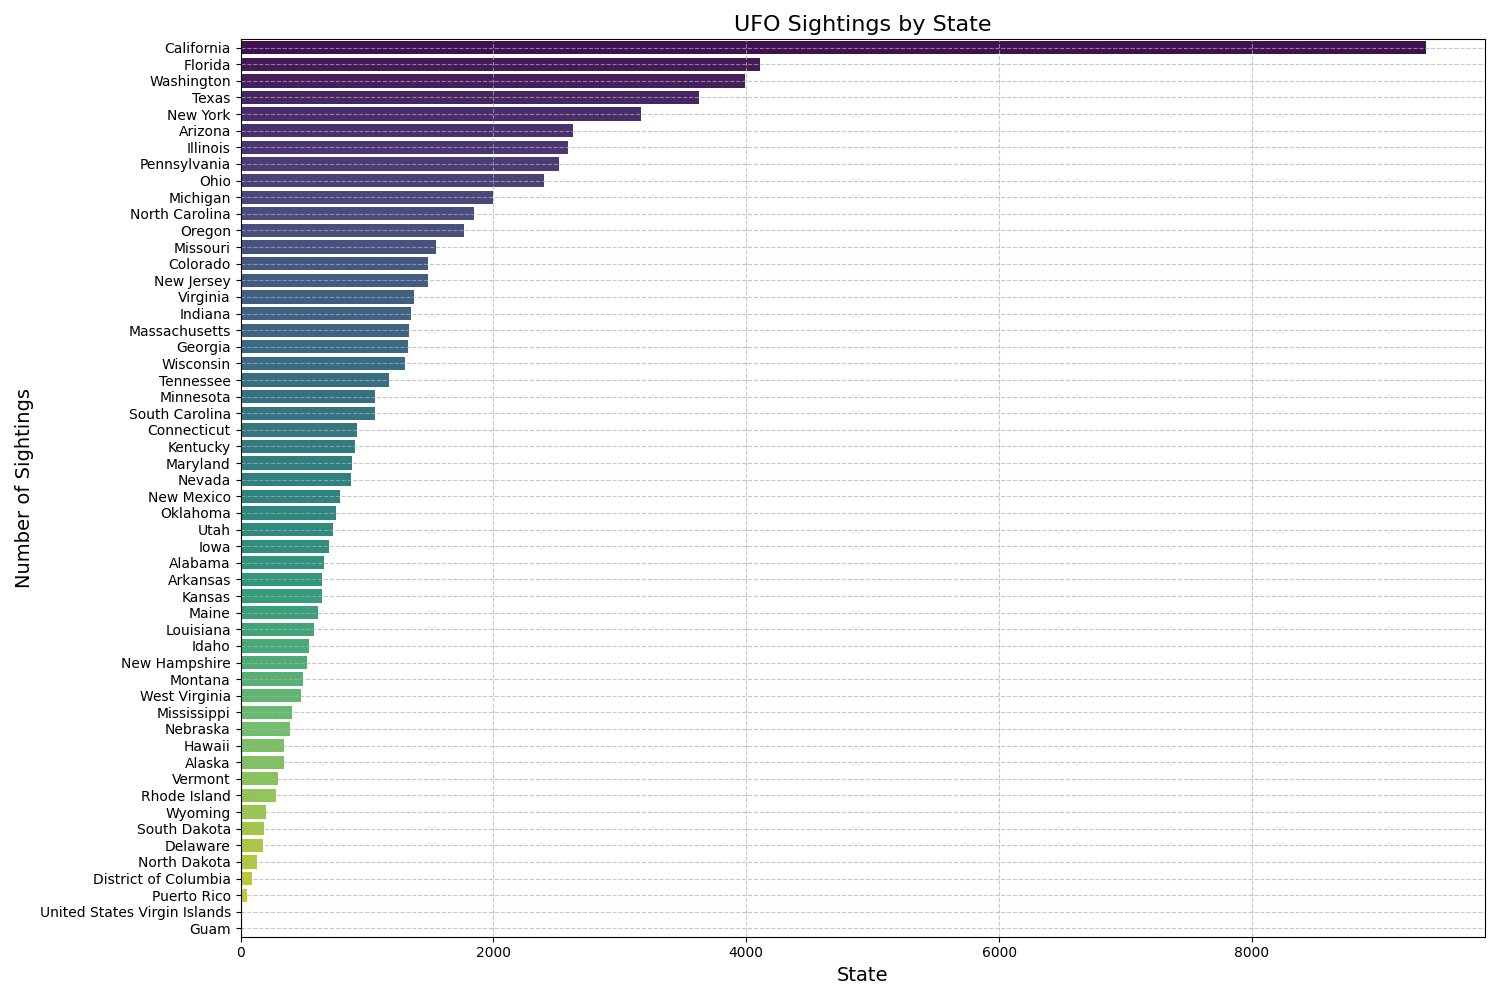
\includegraphics[width=0.8\textwidth]{../images/ufo_sightings_by_state.png}
\caption{Počet pozorování UFO podle států}
\end{figure}

\subsection{Distribuce délky pozorování}
\begin{itemize}
    \item Výstup: histogram délky pozorování UFO v sekundách.
\end{itemize}

\begin{figure}[h]
\centering
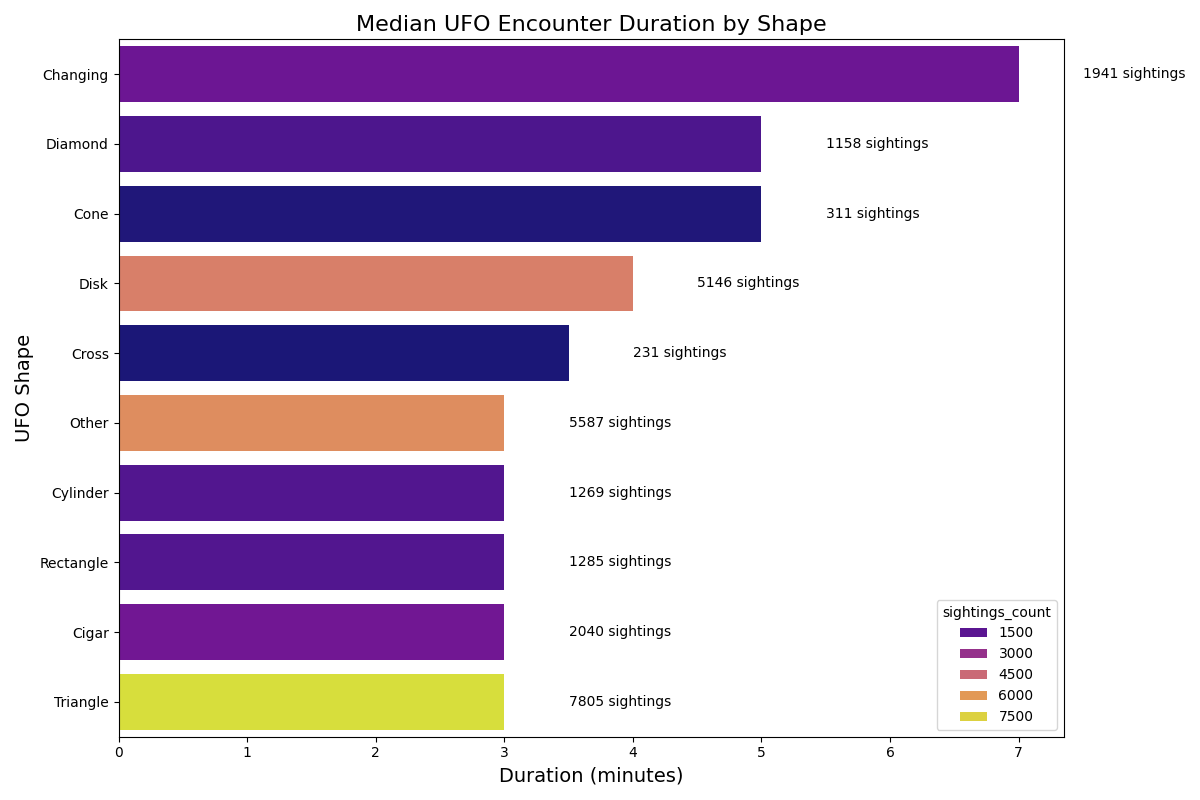
\includegraphics[width=0.8\textwidth]{../images/ufo_encounter_duration.png}
\caption{Délka pozorování UFO}
\end{figure}

\subsection{Pozorování v průběhu dne}
\begin{itemize}
    \item Výstup: graf ukazující počet pozorování v různých hodinách dne.
\end{itemize}

\begin{figure}[h]
\centering
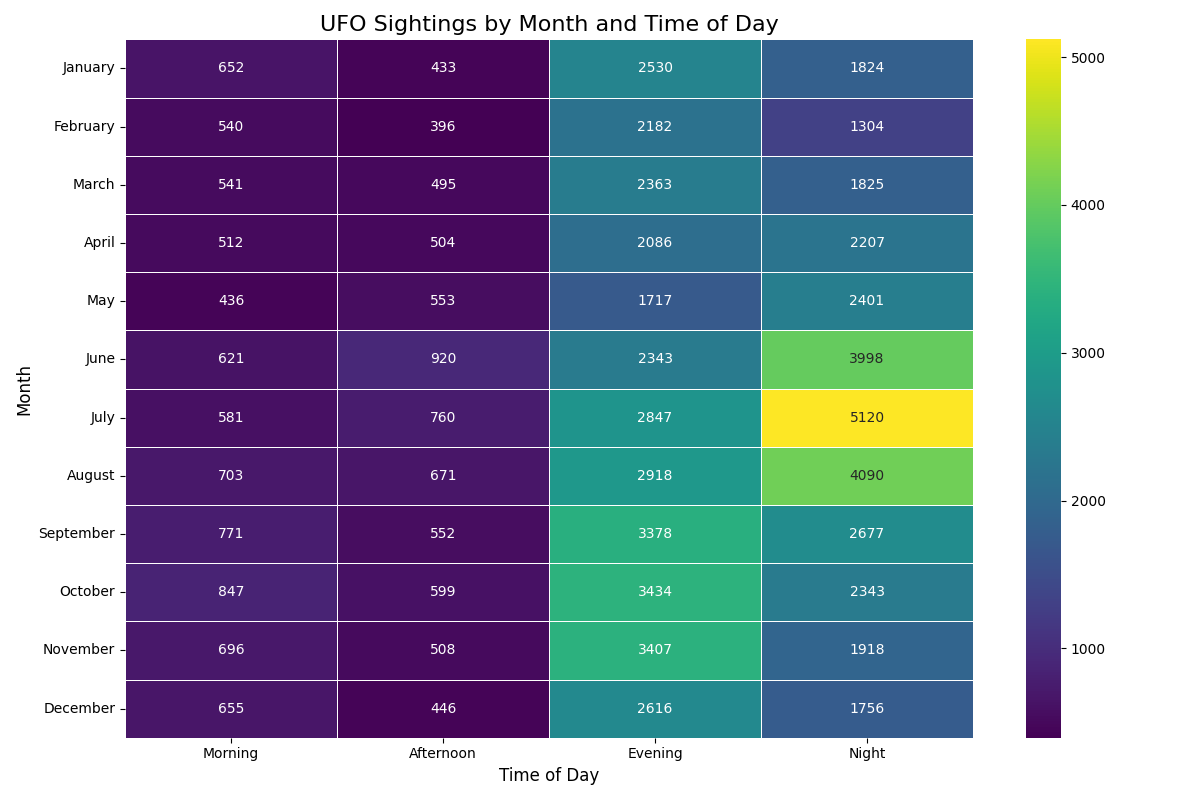
\includegraphics[width=0.8\textwidth]{../images/ufo_sightings_by_time.png}
\caption{Distribuce pozorování podle hodin}
\end{figure}

\section{Data mining}
Pro analýzu dat jsem vyzkoušel několik metod dolování znalostí:

\subsection{Shlukování (Clustering)}
Použil jsem metodu K-Means clusteringu k identifikaci oblastí s častým výskytem pozorování UFO.

\begin{figure}[h]
\centering
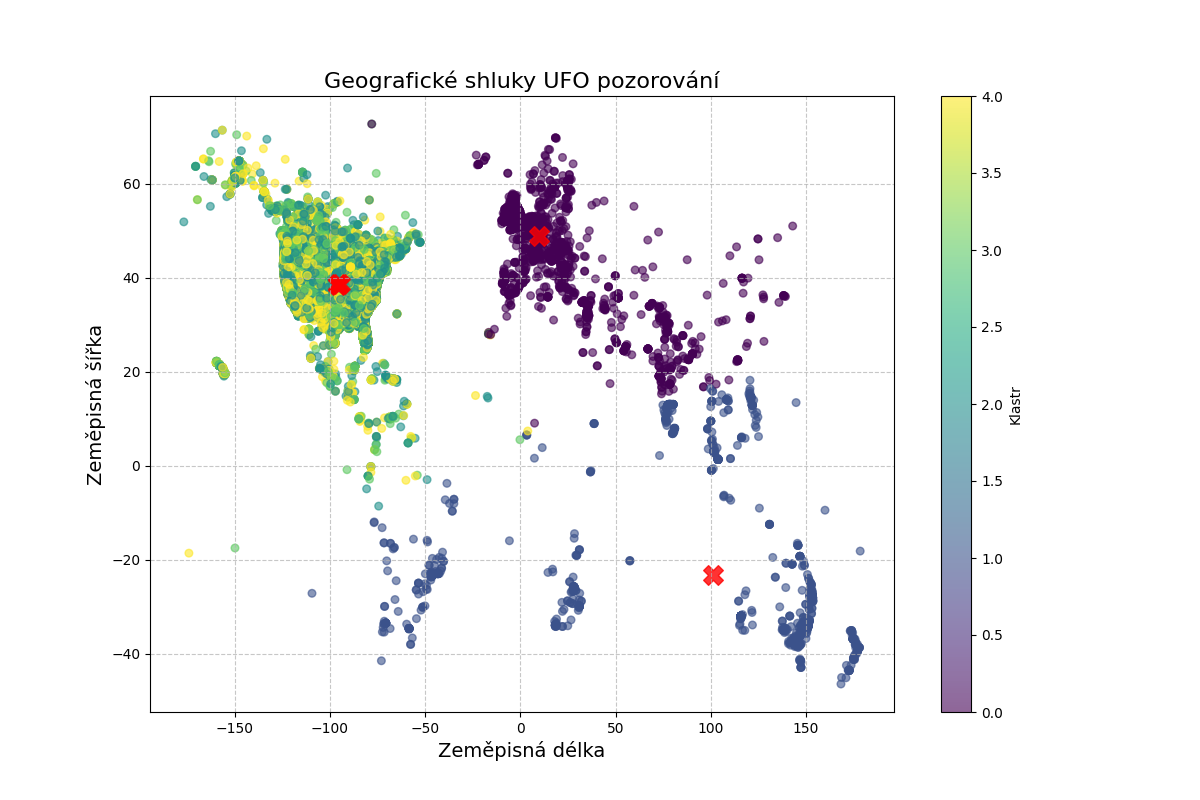
\includegraphics[width=0.8\textwidth]{../images/ufo_clusters_map.png}
\caption{Mapa shluků pozorování UFO}
\end{figure}

\subsection{Asociační pravidla}
Analyzoval jsem textová data z popisů pozorování a hledal časté kombinace slov.

\begin{figure}[h]
\centering
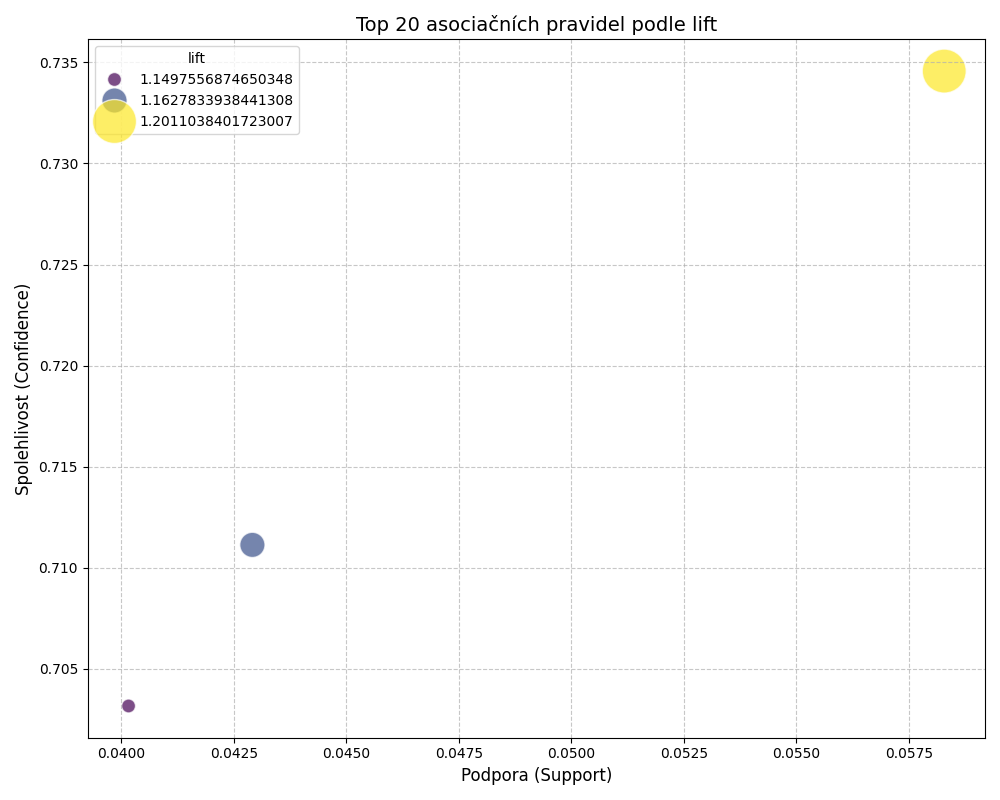
\includegraphics[width=0.8\textwidth]{../images/ufo_association_rules.png}
\caption{Asociační pravidla z popisů pozorování}
\end{figure}

\section{Závěr}
V projektu jsem úspěšně:
\begin{itemize}
    \item nainstaloval a využil DuckDB pro OLAP analýzy,
    \item vytvořil datový sklad ve struktuře hvězdy,
    \item provedl analýzy nad daty pomocí SQL dotazů a Pythonu,
    \item aplikoval metody dolování dat (shlukování, asociační pravidla).
\end{itemize}

Projekt je kompletně připraven v repozitáři a doplněn o vizualizace výsledků.

\end{document}
